\usepackage{amsmath}
\usepackage{amssymb}
\usepackage{xcolor}
\definecolor{dark-red}{rgb}{0.7,0.25,0.25}
\definecolor{dark-blue}{rgb}{0.15,0.15,0.55}
\definecolor{medium-blue}{rgb}{0,0,0.65}

\usepackage{tikz}
\usetikzlibrary{cd}
\usetikzlibrary{knots}
\usetikzlibrary{calc}
\usetikzlibrary{matrix}
\usetikzlibrary{arrows,backgrounds,patterns,scopes,external,hobby,
    decorations.pathreplacing,
    decorations.pathmorphing
}
\usepackage{graphicx}
\usepackage{fullpage}
\usepackage[T1]{fontenc}
\usepackage[final]{microtype}
\usepackage{libertine}
\usepackage[libertine]{newtxmath}
\usepackage{ifthen}

\usepackage{pdfpages}

\usepackage[pdftex,plainpages=false,hypertexnames=false,pdfpagelabels,breaklinks]{hyperref}
\hypersetup{
   colorlinks, linkcolor={purple},
   citecolor={medium-blue}, urlcolor={medium-blue}
}
\urlstyle{same}

\newcommand{\mathfig}[2]{{\hspace{-3pt}\begin{array}{c}%
  \raisebox{-2.5pt}{\includegraphics[width=#1\textwidth]{#2}}%
\end{array}\hspace{-3pt}}}

\newcommand{\arxiv}[1]{\href{https://arxiv.org/abs/#1}{\small  arXiv:#1}}

\newcommand{\nn}[1]{{\color{red} [[#1]]}}

% tricky way to iterate macros over a list
\def\semicolon{;}
\def\applytolist#1{
    \expandafter\def\csname multi#1\endcsname##1{
        \def\multiack{##1}\ifx\multiack\semicolon
            \def\next{\relax}
        \else
            \csname #1\endcsname{##1}
            \def\next{\csname multi#1\endcsname}
        \fi
        \next}
    \csname multi#1\endcsname}

% \def\cA{{\cal A}} for A..Z
\def\calc#1{\expandafter\def\csname c#1\endcsname{{\mathcal #1}}}
\applytolist{calc}QWERTYUIOPLKJHGFDSAZXCVBNM;
% \def\bbA{{\mathbb A}} for A..Z
\def\bbc#1{\expandafter\def\csname bb#1\endcsname{{\mathbb #1}}}
\applytolist{bbc}QWERTYUIOPLKJHGFDSAZXCVBNM;
% \def\bfA{{\mathbf A}} for A..Z
\def\bfc#1{\expandafter\def\csname bf#1\endcsname{{\mathbf #1}}}
\applytolist{bfc}QWERTYUIOPLKJHGFDSAZXCVBNM;

\newcommand{\Kar}{\operatorname{Kar}}
\newcommand{\Obj}{\operatorname{Obj}}
\newcommand{\Fun}{\operatorname{Fun}}
\newcommand{\op}{\operatorname{op}}
\newcommand{\Set}{\mathsf{Set}}
\renewcommand{\Vec}{\mathsf{Vec}}
\newcommand{\fdVec}{\mathsf{fdVec}}
\newcommand{\Rep}{\mathsf{Rep}}

\newcommand{\braidcross}{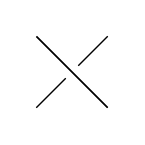
\begin{tikzpicture}[baseline=-0.5ex,scale=0.8]
    \draw (45:.8cm) -- (-135:.8cm);
    \draw[line width=1mm,white,double=black] (-45:.8cm) -- (135:.8cm);
\end{tikzpicture}}
\newcommand{\invbraidcross}{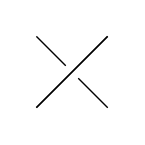
\begin{tikzpicture}[baseline=-0.5ex,scale=0.8]
    \draw (-45:.8cm) -- (135:.8cm);
    \draw[line width=1mm,white,double=black] (45:.8cm) -- (-135:.8cm);
\end{tikzpicture}}
\newcommand{\cupcap}{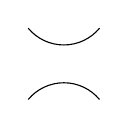
\begin{tikzpicture}[baseline=-0.5ex,scale=0.8]
    \draw (45:.8cm) to [curve through=(90:.3cm)] (135:.8cm);
    \draw (-45:.8cm) to [curve through=(-90:.3cm)] (-135:.8cm);
\end{tikzpicture}}

\newcommand{\twostrandid}{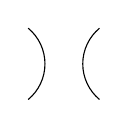
\begin{tikzpicture}[baseline=-0.5ex,rotate=90,scale=0.8]
    \draw (45:.8cm) to [curve through=(90:.3cm)] (135:.8cm);
    \draw (-45:.8cm) to [curve through=(-90:.3cm)] (-135:.8cm);
\end{tikzpicture}}